\chapter{Design Challenges \& Decisions}
\label{sec:design_challenges_and_decisions}

In this chapter we first detail how we determined the subset that our YAML parsers should be able to parse. Afterwards we describe the mapping between YAML and Elektra’s \cc{KeySet} structure. In the last part we then explain the challenges we faced implementing the parser plugins and describe the additional plugins we created to improve the YAML support of Elektra.

\section{YAML Subset}

The \glstext{YAML} standard is extensive. The document describing the serialization language includes about 200 parameterized \gls{BNF} grammar rules~\cite{ben2009yaml}. To simplify the parser development we decided to first determine a subset of \glstext{YAML} that is useful for storing configuration data. For this purpose we discussed the language with other Elektra developers.

\subsection{Method}

We used a requirement analysis to determine useful YAML features. For that purpose we created a \href{https://github.com/sanssecours/YAML-Presentation/blob/master/Questionnaire.md}{questionnaire} that lists YAML features. For each feature we added a checkbox that a participant should check, if they deemed it useful for a YAML subset that stores configuration data. We also added one free form field participants could use to specify additional data types they think should be supported. Since YAML is a complex language we introduced the \glstext{YAML} syntax in a \href{https://github.com/sanssecours/YAML-Presentation/releases/download/v1.0/Presentation.pdf}{presentation} to the Elektra developers first. After we talked about a certain part of YAML, we answered questions the participants had about the information presented so far. Afterwards we asked the participants to fill in the parts of the questionnaire about the newly introduced feature set.

\subsection{Participants}

Nine people participated in the requirement analysis. All of the participants were at least partially familiar with Elektra. Some also had previous experience with \glstext{YAML}. Seven of them listened to the presentation, while one participant was late and another one participated via email. The email participant received a copy of the presentation slides and the questionnaire.

\subsection{Results}

In the following bar charts the term “Yes” refers to a checked box for the specific feature. The term “?” means that the participant did not know enough about a part of \glstext{YAML} and therefore marked the checkbox for one feature, or the heading for multiple features, with a question mark. The value before the term “No” specifies the number of unchecked boxes minus the number of boxes marked with “?”.

\subsubsection{Scalars}

\paragraph{Flow Scalars}

\begin{figure}[H]
  \begin{minipage}[t]{0.48\textwidth}
    \vspace{0pt}
    \begin{bchart}[max=9, width=0.85\textwidth]
      \bcbar[text=3, value=Yes, color=orange]{3}
      \bcbar[text=6, value=No, color=Aqua]{6}
    \end{bchart}
  \end{minipage}
  \begin{minipage}[t]{0.48\textwidth}
    \vspace{0pt}
    \begin{yamlcode}
      Plain String
    \end{yamlcode}
  \end{minipage}
  \caption{Plain Flow Scalar}
\end{figure}

\begin{figure}[H]
  \begin{minipage}[t]{0.48\textwidth}
    \vspace{0pt}
    \begin{bchart}[max=9, width=0.85\textwidth]
      \bcbar[text=2, value=Yes, color=orange]{2}
      \bcbar[text=7, value=No, color=Aqua]{7}
    \end{bchart}
  \end{minipage}
  \begin{minipage}[t]{0.48\textwidth}
    \vspace{0pt}
    \begin{yamlcode}
      'Single Quoted ''String'''
    \end{yamlcode}
  \end{minipage}
  \caption{Single Quoted Flow Scalar}
\end{figure}

\begin{figure}[H]
  \begin{minipage}[t]{0.48\textwidth}
    \vspace{0pt}
    \begin{bchart}[max=9, width=0.85\textwidth]
      \bcbar[text=8, value=Yes, color=orange]{8}
      \bcbar[text=1, value=No, color=Aqua]{1}
    \end{bchart}
  \end{minipage}
  \begin{minipage}[t]{0.48\textwidth}
    \vspace{0pt}
    \begin{yamlcode}
      "Double\n Quoted\n \"String\""
    \end{yamlcode}
  \end{minipage}
  \caption{Double Quoted Flow Scalar}
\end{figure}

\paragraph{Block Scalars}

\begin{figure}[H]
  \begin{minipage}[t]{0.48\textwidth}
    \vspace{0pt}
    \begin{bchart}[max=9, width=0.85\textwidth]
      \bcbar[text=2, value=Yes, color=orange]{2}
      \bcbar[text=6, value=No, color=Aqua]{6}
      \bcbar[text=1, value=?, color=DarkTurquoise]{1}
    \end{bchart}
  \end{minipage}
  \begin{minipage}[t]{0.48\textwidth}
    \vspace{0pt}
    \begin{yamlcode}
      > # "Folded Style"
        Folded
        Style
    \end{yamlcode}
  \end{minipage}
  \caption{Folded Block Scalar}
\end{figure}

\begin{figure}[H]
  \begin{minipage}[t]{0.48\textwidth}
    \vspace{0pt}
    \begin{bchart}[max=9, width=0.85\textwidth]
      \bcbar[text=2, value=Yes, color=orange]{2}
      \bcbar[text=6, value=No, color=Aqua]{6}
      \bcbar[text=1, value=?, color=DarkTurquoise]{1}
    \end{bchart}
  \end{minipage}
  \begin{minipage}[t]{0.48\textwidth}
    \vspace{0pt}
    \begin{yamlcode}
      | # "Literal\nStyle"
        Literal
        Style
    \end{yamlcode}
  \end{minipage}
  \caption{Literal Block Scalar}
\end{figure}

\begin{figure}[H]
  \begin{minipage}[t]{0.48\textwidth}
    \vspace{0pt}
    \begin{bchart}[max=9, width=0.85\textwidth]
      \bcbar[text=1, value=Yes, color=orange]{1}
      \bcbar[text=7, value=No, color=Aqua]{7}
      \bcbar[text=1, value=?, color=DarkTurquoise]{1}
    \end{bchart}
  \end{minipage}
  \begin{minipage}[t]{0.48\textwidth}
    \vspace{0pt}
    \begin{yamlcode*}{showspaces, spacecolor = lightgray, space=·}
      >1 # "  1 Space Indentation"
         1 Space Indentation
    \end{yamlcode*}
  \end{minipage}
  \caption{Indentation Header}
\end{figure}

\begin{figure}[H]
  \begin{minipage}[t]{0.48\textwidth}
    \vspace{0pt}
    \begin{bchart}[max=9, width=0.85\textwidth]
      \bcbar[text=0, value=$\quad$Yes, color=orange]{0}
      \bcbar[text=8, value=No, color=Aqua]{8}
      \bcbar[text=1, value=?, color=DarkTurquoise]{1}
    \end{bchart}
  \end{minipage}
  \begin{minipage}[t]{0.48\textwidth}
    \vspace{0pt}
    \begin{yamlcode*}{showspaces, spacecolor = lightgray, space=·, escapeinside=||}
      >- # "No Trailing Whitespace"
         No Trailing Whitespace
        | |
        | |
      # ⬆️ Newlines Above Stripped
    \end{yamlcode*}
  \end{minipage}
  \caption{Chomping Header}
\end{figure}

\subsubsection{Lists}

\begin{figure}[H]
  \begin{minipage}[t]{0.48\textwidth}
    \vspace{0pt}
    \begin{bchart}[max=9, width=0.85\textwidth]
      \bcbar[text=5, value=Yes, color=orange]{5}
      \bcbar[text=4, value=No, color=Aqua]{4}
    \end{bchart}
  \end{minipage}
  \begin{minipage}[t]{0.48\textwidth}
    \vspace{0pt}
    \begin{yamlcode}
      [🍎, 🍊,
        [Sugar, Eggs, Chocolate]
      ]
    \end{yamlcode}
  \end{minipage}
  \caption{Flow Style}
\end{figure}

\begin{figure}[H]
  \begin{minipage}[t]{0.48\textwidth}
    \vspace{0pt}
    \begin{bchart}[max=9, width=0.85\textwidth]
      \bcbar[text=7, value=Yes, color=orange]{7}
      \bcbar[text=2, value=No, color=Aqua]{2}
    \end{bchart}
  \end{minipage}
  \begin{minipage}[t]{0.48\textwidth}
    \vspace{0pt}
    \begin{yamlcode}
      - 🍎
      - 🍊
      - - Sugar
        - Eggs
        - Chocolate
    \end{yamlcode}
  \end{minipage}
  \caption{Block Style}
\end{figure}

\subsubsection{Mappings}

\begin{figure}[H]
  \begin{minipage}[t]{0.48\textwidth}
    \vspace{0pt}
    \begin{bchart}[max=9, width=0.85\textwidth]
      \bcbar[text=5, value=Yes, color=orange]{5}
      \bcbar[text=4, value=No, color=Aqua]{4}
    \end{bchart}
  \end{minipage}
  \begin{minipage}[t]{0.48\textwidth}
    \vspace{0pt}
    \begin{yamlcode}
      { Austria: Vienna,
        South Africa: {
          Executive: Pretoria,
          Judicial: Bloemfontein,
          Legislative: Cape Town }
      }
    \end{yamlcode}
  \end{minipage}
  \caption{Flow Style}
\end{figure}

\begin{figure}[H]
  \begin{minipage}[t]{0.48\textwidth}
    \vspace{0pt}
    \begin{bchart}[max=9, width=0.85\textwidth]
      \bcbar[text=7, value=Yes, color=orange]{7}
      \bcbar[text=2, value=No, color=Aqua]{2}
    \end{bchart}
  \end{minipage}
  \begin{minipage}[t]{0.48\textwidth}
    \vspace{0pt}
    \begin{yamlcode}
      Austria: Vienna
      South Africa:
        Executive:   Pretoria
        Judicial:    Bloemfontein
        Legislative: Cape Town
    \end{yamlcode}
  \end{minipage}
  \caption{Block Style}
\end{figure}

\begin{figure}[H]
  \begin{minipage}[t]{0.48\textwidth}
    \vspace{0pt}
    \begin{bchart}[max=9, width=0.85\textwidth]
      \bcbar[text=0, value=$\quad$Yes, color=orange]{0}
      \bcbar[text=9, value=No, color=Aqua]{9}
    \end{bchart}
  \end{minipage}
  \begin{minipage}[t]{0.48\textwidth}
    \vspace{0pt}
    \begin{yamlcode}
      ?
      - { 'pretty': complex key }
      - - 😱
      - Still part of the key
      : value
    \end{yamlcode}
  \end{minipage}
  \caption{Support for Complex Keys}
\end{figure}

\subsubsection{Multiple Documents}

\begin{figure}[H]
  \begin{minipage}[t]{0.48\textwidth}
    \vspace{0pt}
    \begin{bchart}[max=9, width=0.85\textwidth]
      \bcbar[text=0, value=$\quad$Yes, color=orange]{0}
      \bcbar[text=9, value=No, color=Aqua]{9}
    \end{bchart}
  \end{minipage}
  \begin{minipage}[t]{0.48\textwidth}
    \vspace{0pt}
    \begin{yamlcode}
      "Hello First Document"
      ...
      'Second Document'
      ...
      Third Document
    \end{yamlcode}
  \end{minipage}
  \caption{Support Streams}
\end{figure}

\subsubsection{Types}

\paragraph{Directives}

\begin{figure}[H]
  \begin{minipage}[t]{0.48\textwidth}
    \vspace{0pt}
    \begin{bchart}[max=9, width=0.85\textwidth]
      \bcbar[text=1, value=Yes, color=orange]{1}
      \bcbar[text=7, value=No, color=Aqua]{7}
      \bcbar[text=1, value=?, color=DarkTurquoise]{1}
    \end{bchart}
  \end{minipage}
  \begin{minipage}[t]{0.48\textwidth}
    \vspace{0pt}
    \begin{yamlcode}
      %YAML 1.2
    \end{yamlcode}
  \end{minipage}
  \caption{\glstext{YAML} Version}
\end{figure}

\begin{figure}[H]
  \begin{minipage}[t]{0.48\textwidth}
    \vspace{0pt}
    \begin{bchart}[max=9, width=0.85\textwidth]
      \bcbar[text=3, value=Yes, color=orange]{3}
      \bcbar[text=5, value=No, color=Aqua]{5}
      \bcbar[text=1, value=?, color=DarkTurquoise]{1}
    \end{bchart}
  \end{minipage}
  \begin{minipage}[t]{0.48\textwidth}
    \vspace{0pt}
    \begin{yamlcode}
      %TAG !      tag:yaml.org,2002:
      %TAG !!     tag:yaml.org,2002:
      %TAG !name! tag:yaml.org,2002:
      ---
    \end{yamlcode}
  \end{minipage}
  \caption{Tag Handle Definition}
\end{figure}

\begin{figure}[H]
  \begin{minipage}[t]{0.48\textwidth}
    \vspace{0pt}
    \begin{bchart}[max=9, width=0.85\textwidth]
      \bcbar[text=2, value=Yes, color=orange]{2}
      \bcbar[text=6, value=No, color=Aqua]{6}
      \bcbar[text=1, value=?, color=DarkTurquoise]{1}
    \end{bchart}
  \end{minipage}
  \begin{minipage}[t]{0.48\textwidth}
    \vspace{0pt}
    \begin{yamlcode}
      %TAG !name! tag:yaml.org,2002:
      ---
      !name!str 6 # "6"
    \end{yamlcode}
  \end{minipage}
  \caption{Named Tag Handle}
\end{figure}

\paragraph{Tags}

\subparagraph{Tag Shorthands}

\begin{figure}[H]
  \begin{minipage}[t]{0.48\textwidth}
    \vspace{0pt}
    \begin{bchart}[max=9, width=0.85\textwidth]
      \bcbar[text=4, value=Yes, color=orange]{4}
      \bcbar[text=4, value=No, color=Aqua]{4}
      \bcbar[text=1, value=?, color=DarkTurquoise]{1}
      \bcxlabel{}
    \end{bchart}
  \end{minipage}
  \begin{minipage}[t]{0.48\textwidth}
    \vspace{0pt}
    \begin{yamlcode}
      !suffix value
    \end{yamlcode}
  \end{minipage}
  \caption{Primary Tag Handle}
\end{figure}

\begin{figure}[H]
  \begin{minipage}[t]{0.48\textwidth}
    \vspace{0pt}
    \begin{bchart}[max=9, width=0.85\textwidth]
      \bcbar[text=3, value=Yes, color=orange]{3}
      \bcbar[text=5, value=No, color=Aqua]{5}
      \bcbar[text=1, value=?, color=DarkTurquoise]{1}
    \end{bchart}
  \end{minipage}
  \begin{minipage}[t]{0.48\textwidth}
    \vspace{0pt}
    \begin{yamlcode}
      !!suffix value
    \end{yamlcode}
  \end{minipage}
  \caption{Secondary Tag Handle}
\end{figure}

\begin{figure}[H]
\subparagraph{Verbatim Tags}
  \begin{minipage}[t]{0.48\textwidth}
    \vspace{0pt}
    \begin{bchart}[max=9, width=0.85\textwidth]
      \bcbar[text=0, value=$\quad$Yes, color=orange]{0}
      \bcbar[text=8, value=No, color=Aqua]{8}
      \bcbar[text=1, value=?, color=DarkTurquoise]{1}
    \end{bchart}
  \end{minipage}
  \begin{minipage}[t]{0.48\textwidth}
    \vspace{0pt}
    \begin{yamlcode}
      !<!ruby/object:Set> value
    \end{yamlcode}
  \end{minipage}
  \caption{Local Verbatim Tags}
\end{figure}

\begin{figure}[H]
  \begin{minipage}[t]{0.48\textwidth}
    \vspace{0pt}
    \begin{bchart}[max=9, width=0.85\textwidth]
      \bcbar[text=0, value=$\quad$Yes, color=orange]{0}
      \bcbar[text=8, value=No, color=Aqua]{8}
      \bcbar[text=1, value=?, color=DarkTurquoise]{1}
    \end{bchart}
  \end{minipage}
  \begin{minipage}[t]{0.48\textwidth}
    \vspace{0pt}
    \begin{yamlcode}
      !<tag:yaml.org,2002:str> value
    \end{yamlcode}
  \end{minipage}
  \caption{Global Verbatim Tags}
\end{figure}

\subparagraph{Other Tags}

\begin{figure}[H]
  \begin{minipage}[t]{0.48\textwidth}
    \vspace{0pt}
    \begin{bchart}[max=9, width=0.85\textwidth]
      \bcbar[text=0, value=$\quad$Yes, color=orange]{0}
      \bcbar[text=8, value=No, color=Aqua]{8}
      \bcbar[text=1, value=?, color=DarkTurquoise]{1}
    \end{bchart}
  \end{minipage}
  \begin{minipage}[t]{0.48\textwidth}
    \vspace{0pt}
    \begin{yamlcode}
      ! value
    \end{yamlcode}
  \end{minipage}
  \caption{Non-Specific Tag}
\end{figure}

\paragraph{Schemas}

\textbf{Remark:} One participant checked the box for the core schema without ticking the boxes for the failsafe and \gls{JSON} schema. Since the core schema is an extended superset of the other two schemas, we counted the participants answers as a “Yes” vote for the failsafe and \gls{JSON} schema.

\begin{figure}[H]
  \begin{minipage}[t]{0.48\textwidth}
    \vspace{0pt}
    \begin{bchart}[max=9, width=0.85\textwidth]
      \bcbar[text=5, value=Yes, color=orange]{5}
      \bcbar[text=3, value=No, color=Aqua]{3}
      \bcbar[text=1, value=?, color=DarkTurquoise]{1}
      \bcxlabel{}
    \end{bchart}
  \end{minipage}
  \begin{minipage}[t]{0.48\textwidth}
    \vspace{0pt}
    \begin{itemize}
      \item String
      \item Sequence
      \item Map
    \end{itemize}
  \end{minipage}
  \caption{Failsafe Schema}
\end{figure}

\begin{figure}[H]
  \begin{minipage}[t]{0.48\textwidth}
    \vspace{0pt}
    \begin{bchart}[max=9, width=0.85\textwidth]
      \bcbar[text=5, value=Yes, color=orange]{5}
      \bcbar[text=3, value=No, color=Aqua]{3}
      \bcbar[text=1, value=?, color=DarkTurquoise]{1}
    \end{bchart}
  \end{minipage}
  \begin{minipage}[t]{0.48\textwidth}
    \vspace{0pt}
    Failsafe Schema + \gls{JSON} Types:
    \begin{minipage}[t]{2cm}
      \begin{itemize}[leftmargin=*]
        \item Null
        \item Boolean
        \item Integer
        \item Float
      \end{itemize}
    \end{minipage}
  \end{minipage}
  \caption{JSON Schema}
\end{figure}

\begin{figure}[H]
  \begin{minipage}[t]{0.48\textwidth}
    \vspace{0pt}
    \begin{bchart}[max=9, width=0.85\textwidth]
      \bcbar[text=3, value=Yes, color=orange]{3}
      \bcbar[text=5, value=No, color=Aqua]{5}
      \bcbar[text=1, value=?, color=DarkTurquoise]{1}
    \end{bchart}
  \end{minipage}
  \begin{minipage}[t]{0.48\textwidth}
    \vspace{0pt}
    \gls{JSON} Schema and
      \vspace{-0.5cm}
      \begin{itemize}
        \item Octal/Hex: \yaml{0o123}, \yaml{0xfefe}
        \item Multiple Notations for same value:
              \yaml{null}, \yaml{Null}, \yaml{~}
      \end{itemize}
  \end{minipage}
  \caption{Core Schema}
\end{figure}

\begin{figure}[H]
  \begin{minipage}[t]{0.48\textwidth}
    \vspace{0pt}
    \begin{bchart}[max=9, width=0.85\textwidth]
      \bcbar[text=3, value=Yes, color=orange]{3}
      \bcbar[text=5, value=No, color=Aqua]{5}
      \bcbar[text=1, value=?, color=DarkTurquoise]{1}
    \end{bchart}
  \end{minipage}
  \begin{minipage}[t]{0.48\textwidth}
    \vspace{0pt}
    \begin{itemize}
      \item Ordered Map
      \item Set
      \item Binary
      \item Time
      \item …
    \end{itemize}
  \end{minipage}
  \caption{Additional Types}
\end{figure}

\subparagraph{Which Additional Types:}
\begin{itemize}
  \item “” (No answer)
  \item “binary”
  \item “date (but implemented in plugins)”
\end{itemize}

\subsubsection{References}

\begin{figure}[H]
  \begin{minipage}[t]{0.48\textwidth}
    \vspace{0pt}
    \begin{bchart}[max=9, width=0.85\textwidth]
      \bcbar[text=7, value=Yes, color=orange]{7}
      \bcbar[text=2, value=No, color=Aqua]{2}
    \end{bchart}
  \end{minipage}
  \begin{minipage}[t]{0.48\textwidth}
    \vspace{0pt}
    \begin{yamlcode}
      flowers: &flowers
        🌳🌸🌼
      garden:
        - *flowers # 🌳🌸🌼
        - *flowers # 🌳🌸🌼
    \end{yamlcode}
  \end{minipage}
  \caption{Support Anchors \& Aliases}
\end{figure}

\subsection{Interpretation}

The results of the survey showed that the participants preferred double quoted flow scalars over single quoted and plain scalars. A reasons for this could be that those scalars are familiar from other languages such as C, and that they are able to express arbitrary data. Asked about block scalar styles most of the Elektra developers did not think that any of the two styles were necessary.

In contrast to the decision about block scalars, the participants preferred the block styles of sequences and mappings (\glspl{collection}) over the respective flow style. However, they also decided that a useful \glstext{YAML} subset should include flow \glspl{collection}.

The Elektra developers decided against most of the specialized type features of \glstext{YAML}. Only the result count for and against primary tag handles resulted in a draw.

The questions about general type support (schemas) showed that a minimal \glstext{YAML} subset should include all types of the \gls{JSON} Schema.

One of the few specialized features deemed necessary by the participants were anchors and aliases. These two elements can be used to reference the same data multiple times in the same document.

\subsubsection{Summary}

The list below contains a summary of the \glstext{YAML} features that should be part of a minimal \glstext{YAML} subset according to the results of the discussion:

\begin{itemize}
  \item double quoted flow scalars,
  \item block and flow collections,
  \item \gls{JSON} schema,
  \item primary tag handle, and
  \item references.
\end{itemize}

\subsubsection{Problems of the Survey}

The questionnaire was done in an early phase of the thesis to gather some insights about YAML features for configuration data. While it showed some interesting results, we noticed problems that made the results unusable for the implementation phase.

One of these problems is the small sample size. With only 9 participants the maximum margin of error for a $95\%$ confidence interval is approximately $32\%$:

% https://www.cs.mcgill.ca/~rwest/wikispeedia/wpcd/wp/m/Margin_of_error.htm
\[
  SE =
  1.96·\sqrt{\frac{\frac{4}{9}·\left(1-\frac{4}{9}\right)}{9}} ≅
  0.32 (32\%)
\]

Another problem even applies to results with a high percentage for one of the options, when the margin of error is smaller. The participants were not experts in the area of parsing. At the time of the survey this was also true for the author of the thesis. As a consequence the results included features, such as references, that are not that interesting from a parsing standpoint, but would require significant work in the core of Elektra, something that we consider out of the scope of the thesis.

\subsubsection{Decision}
\label{sec:discussion_decision}

In the end the decision about the implemented YAML features was largely a results of the implementation phase (see Section~\nameref{sec:parsers}). We built the parser starting with smaller features such as scalar support and then added additional features. We decided to implement the following list of items for the \glstext{YAML} subset:

\begin{itemize}
  \item double quoted scalars,
  \item single quoted scalars,
  \item plain flow scalars,
  \item block collections, and
  \item core schema (no tag support).
\end{itemize}

\section{Mapping Between Elektra’s Data Types and YAML}
\label{sec:mapping_elektra_yaml}

\begin{sloppypar}
  There are basically two more or less obvious solutions to map data between Elektra’s \cc{KeySet} structure and a \glstext{YAML} file. Since a \cc{KeySet} behaves similar to a map (see also section~“\nameref{sec:keyset}”), connecting a certain key to a certain value, we could use \glstext{YAML}’s map type directly.
\end{sloppypar}

\begin{figure}
  \centering
    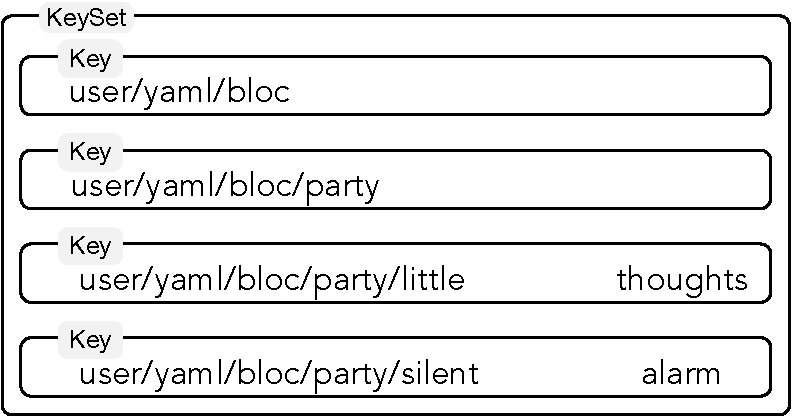
\includegraphics[width=.5\textwidth]{Keys}
  \caption{An exemplary \cc{KeySet}}
  \label{fig:keys}
\end{figure}

For example, the \cc{KeySet} shown in Figure~\ref{fig:keys} would then map to the following \glstext{YAML} data, if we use \code{user/yaml} as mountpoint:

\begin{yamlcode}
  bloc:
  bloc/party:
  bloc/party/little: "thoughts"
  bloc/party/silent: "alarm"
\end{yamlcode}

. As we can see the resulting \glstext{YAML} file contains quite a lot of redundant data.

In our second solution we take the hierarchical nature of the database into account and split on each part of a key. The result of this approach is the following \glstext{YAML} file:

\begin{yamlcode}
  bloc:
    party:
      little: "thoughts"
      silent: "alarm"
\end{yamlcode}

. The second solution removes unwanted redundancy and reflects the hierarchy much better. However, the approach also has an obvious downside: What happens if we want to store a value in \code{user/yaml/bloc} or \code{user/yaml/bloc/party}? To answer this question, let us look at a tree representing the \glstext{YAML} data from above.

As we can see in Figure~\ref{fig:tree} the only nodes that store values are the leaves of the tree. Let us assume we also want to store the value \code{chain} in \code{user/yaml/bloc}. Figure~\ref{fig:tree_extended} shows the resulting tree.

\begin{figure}[H]
  \centering
  \begin{subfigure}[t]{.4\textwidth}
    \centering
    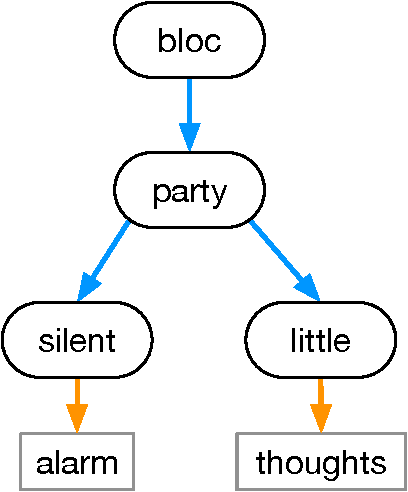
\includegraphics[height=4cm]{Tree}
    \caption{Initial representation}
    \label{fig:tree}
  \end{subfigure}
  \qquad
  \begin{subfigure}[t]{.4\textwidth}
    \centering
    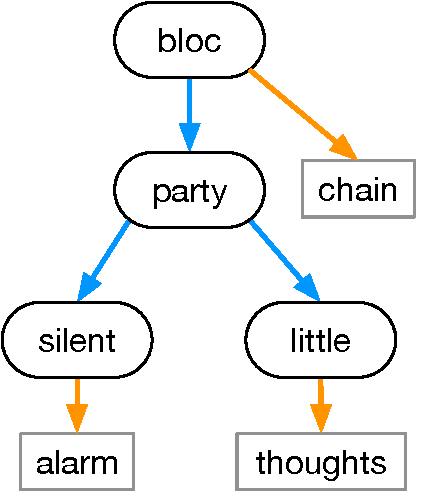
\includegraphics[height=4cm]{TreeExtended}
    \caption{We add an additional value}
    \label{fig:tree_extended}
  \end{subfigure}\\
  \begin{subfigure}[t]{.4\textwidth}
    \centering
    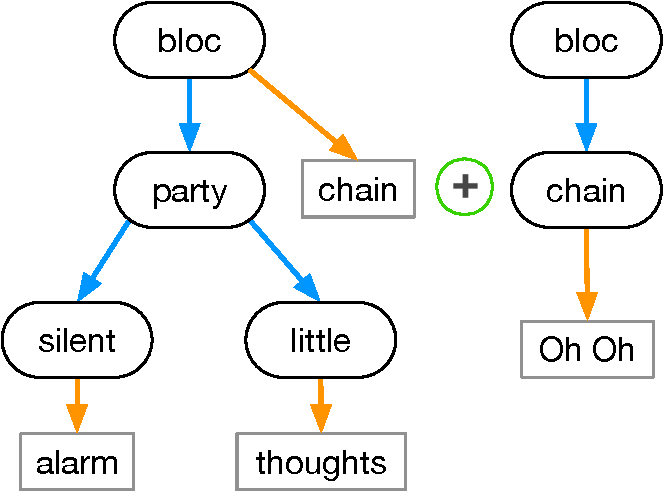
\includegraphics[height=4cm]{TreeExtended+}
    \caption{We add an additional \cc{Key} containing a value}
  \end{subfigure}
  \quad
  \begin{subfigure}[t]{.4\textwidth}
    \centering
    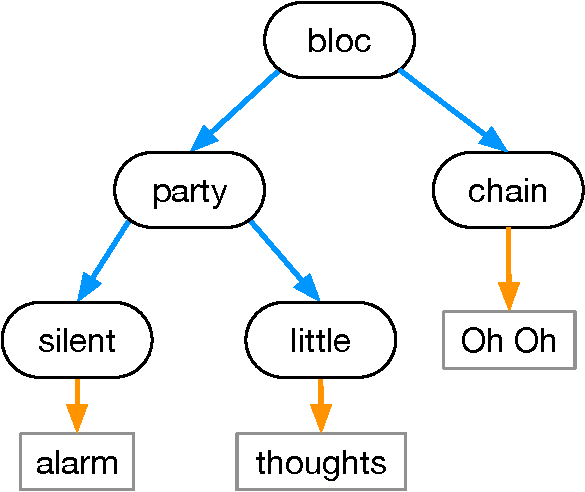
\includegraphics[height=4cm]{TreeExtended++}
    \caption{The new \cc{Key} overwrites the value of the node \code{block}}
    \label{fig:tree_extended++}
  \end{subfigure}
  \caption{The tree-like representation of \glstext{YAML} data shows the problem of adding non-leaf values}
\end{figure}

We could now save \code{chain} as a map key inside \code{bloc}:

\begin{yamlcode}
  bloc:
    chain:
    party:
      little: "thoughts"
      silent: "alarm"
\end{yamlcode}

. However using this approach we are unable to differentiate between the name and the value of a \cc{Key}. For example, if we add a new \cc{Key} with the name \code{user/yaml/bloc/chain} it would just overwrite the value of \code{user/yaml/bloc} (see Figure~\ref{fig:tree_extended++}).

Another option to fix our problem would be to use \glstext{YAML}’s sequence type, and to store the value of a \cc{Key} and the data below the \cc{Key} as first and second element of the sequence:

\begin{yamlcode}
  bloc:
    - chain                 # First element stores value
    - party:                # Second element stores data below
      -                     # `user/yaml/bloc/party` contains no value
      - little: "thoughts"
        silent: "alarm"
\end{yamlcode}

. However, this format is quite complicated. If we add support for Elektra’s array type – mapping arrays to \glstext{YAML} sequences – the situation is even worse.

To solve the problem we use another approach. We reserve the name \yaml{___dirdata} to save values in non-leaf nodes. The code below shows the mapping of our example data:

\begin{yamlcode}
  bloc:
    ___dirdata: "chain"
    party:
      little: "thoughts"
      silent: "alarm"
\end{yamlcode}

. Since we reserved the name \yaml{___dirdata} the value below this key will always be a leaf of the tree.

\subsection{Mapping Arrays}

Since Elektra’s array type and \glstext{YAML} sequences are similar, we want to map between these data types.

\begin{figure}
  \centering
    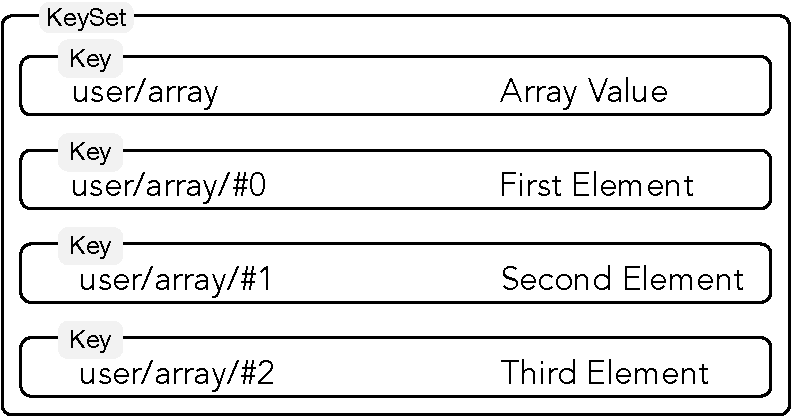
\includegraphics[width=.6\textwidth]{ArrayValue}
  \caption{The \cc{KeySet} above describes an array containing three elements}
  \label{fig:array_value}
\end{figure}

If we use this approach, then the \cc{KeySet} shown in Figure~\ref{fig:array_value} would result in the \glstext{YAML} data:

\begin{yamlcode}
  array:
    - "First Element"
    - "Second Element"
    - "Third Element"
\end{yamlcode}

. We are left with the problem, where to save the data of the \emph{parent} \cc{Key} of the array elements \code{user/array}. We cannot use the same approach as before:

\begin{yamlcode}
  array:
    ___dirdata: "Array Value"
    - "First Element"
    - "Second Element"
    - "Third Element"
\end{yamlcode}

since the result would be a \glstext{YAML} node that is neither sequence nor map. To fix this problem we decided to convert the \yaml{___dirdata} node to a sequence element:

\begin{yamlcode}
  array:
    - "___dirdata: Array Value"
    - "First Element"
    - "Second Element"
    - "Third Element"
\end{yamlcode}

This approach produces valid \glstext{YAML} data and allows us to distinguish between array parents that store values and parents that do not, by checking the first array element for the value prefix \yaml{___dirdata:}.

\section{Parsers}
\label{sec:parsers}

The next section describes some of the implementation challenges we faced when we developed our parsing plugins.

\subsection{Recursive Descent Parser}

The first \href{https://github.com/ElektraInitiative/libelektra/commit/3d2d4644cb08e83f0b3305b8aeae546ada52dfe7}{\glstext{YAML} plugin} we developed used a handwritten recursive descent parser. This technique is quite popular, since there exists a natural correspondence between code and grammar rules. Table~\ref{tab:recursive_descent_correspondence} shows the correspondence between \gls{ABNF} grammar rules and matching C like pseudocode.

\begin{table}[H]
  \begin{center}
    \begin{tabular}{llp{0.48\textwidth}}
      \toprule
      Grammar & Example & Code\\
      \midrule

      \vspace{0cm}
      Terminal
      &
      \vspace{0cm}
      \codebox{
      \texttt{{\color{color02} a}
              {\color{color03} \textbf{=}}
              {\color{color07} "a"}}}
      &
      \vspace{-0.36cm}
      \begin{minted}[autogobble]{c}
        bool a() {
          bool match = getc(file) == 'a';
          if (!match) putc(file);
          return match;
        }
      \end{minted}
      \\

      \vspace{0cm}
      Sequence
      &
      \vspace{0cm}
      \codebox{
      \texttt{{\color{color02} seq}
              {\color{color03} \textbf{=}}
              {\color{color02} rule1 rule2}}}
      &
      \vspace{-0.36cm}
      \begin{minted}[autogobble]{c}
        bool seq() {
          return rule1() && rule2();
        }
      \end{minted}
      \\

      \vspace{0cm}
      Alternative
      &
      \vspace{0cm}
      \codebox{
      \texttt{{\color{color02} seq}
              {\color{color03} \textbf{=}}
              {\color{color02} rule1}
              {\color{color03} /}
              {\color{color02} rule2}}}
      &
      \vspace{-0.36cm}
      \begin{minted}[autogobble]{c}
        bool alt() {
          return rule1() || rule2();
        }
      \end{minted}
      \\

      \bottomrule
    \end{tabular}
  \end{center}
  \caption{Correspondence between grammar rules and code in a recursive descent parser}
  \label{tab:recursive_descent_correspondence}
\end{table}

While Table~\ref{tab:recursive_descent_correspondence} suggest writing a recursive descent parser is trivial, there are many problems that the code above does not take into account.

\begin{description}
  \item [Recognizer Only:] The pseudocode only implements a recognizer for the language. At the end of the parsing process we only know whether the input is part of the language produced by the given grammar or not. Usually we want to \emph{build a data structure}, in our case a \cc{KeySet}, from the given input.

  \item [Error Handling:] The code does not contain any error handling. If a given input contains errors, then the author of the data wants to know \emph{where these errors occurred}. Otherwise she or he has to check the whole input.

  \item [Left Recursion:] If we translate a left recursive rules such as \code{\color{color02} rule1 \color{color03} \textbf{=} \color{color02} rule1 \color{color03} / \color{color02} rule2} using the correspondences given in Table~\ref{tab:recursive_descent_correspondence}, then the resulting code would never terminate. This is the case, since \code{\color{color02} rule1} calls \code{{\color{color02} rule1}}, which then calls \code{\color{color02} rule1}, and so on an so forth (infinite recursion).
\end{description}

All of the problems above apply regardless of the programming language of the parsing code. Since we implemented the recursive descent parser in C, another issue is the error handling in C itself. The language does not provide a native exception handling mechanism. We therefore used the return value to also transfer the error information between functions. This approach is quite cumbersome, since it basically means that we have to check for an error after each function call.

We used C macros to minimize the code overhead and complexity caused by the error handling. Still, for a very small part of the \glstext{YAML} syntax described in the ABNF grammar of Figure~\ref{cod:abnf_recurive_descent} the parser contained about 374 lines of code (counted with \code{cloc} version 1.72). While smaller feature additions, such as supporting multiple key-value pairs instead of only one key-value pair \href{https://github.com/ElektraInitiative/libelektra/commit/17aa7a6ea5d9261287104213dcba67f4d0a0fcbc}{were quite straightforward} (14 additions, 1 deletion), other modifications, such as supporting block styles would take considerable more effort.

Since the first steps with a handwritten recursive descent parser showed that this approach takes considerable effort we decided against extending the first prototype. Instead we chose to use an already existing handwritten \glstext{YAML} parser.

\begin{listing}
  \centering
  \begin{code-boxed}
    {\small
{\color{color02} NEL} {\color{color03} \textbf{=}} {\color{color04} \%x85}{\color{color05} \\}{\color{color02} WSLF}
{\color{color03} \textbf{=}} {\color{color04} \textbf{WSP}} {\color{color03} \textbf{/}}
{\color{color04} \textbf{LF}}{\color{color05} \\\\}{\color{color06} ; Printable
characters from C0 set\\}{\color{color02} printable} {\color{color03} \textbf{=}}
{\color{color04} \textbf{HTAB}} {\color{color03} \textbf{/}} {\color{color04} \textbf{LF}}
{\color{color03} \textbf{/}} {\color{color04} \textbf{CR}}{\color{color05} \\}{\color{color06} ;
Printable ASCII\\}{\color{color02} printable} {\color{color03} \textbf{=/}} {\color{color04} \%x20}{\color{color03} \textbf{-}}{\color{color04} 7e}{\color{color05} \\}{\color{color06} ;
Next Line from C1 set\\}{\color{color02} printable} {\color{color03} \textbf{=/}}
{\color{color02} NEL}{\color{color05} \\}{\color{color06} ; Characters after C1
set -- Surrogate pairs\\}{\color{color02} printable} {\color{color03} \textbf{=/}}
{\color{color04} \%xa0}{\color{color03} \textbf{-}}{\color{color04} d7ff}{\color{color05} \\}{\color{color06} ;
Private use characters -- Replacement character\\}{\color{color02} printable}
{\color{color03} \textbf{=/}} {\color{color04} \%xe00}{\color{color03} \textbf{-}}{\color{color04} fffd}{\color{color05} \\}{\color{color06} ;
All Unicode Character Starting from the Supplementary Multilingual Plain\\}{\color{color02} printable}
{\color{color03} \textbf{=/}} {\color{color04} \%x10000}{\color{color03} \textbf{-}}{\color{color04} 10ffff}{\color{color05} \\\\}{\color{color02} pairs}
{\color{color03} \textbf{=}} {\color{color03} \textbf{*}}{\color{color02} WSLF}
{\color{color07} \texttt{"}\{\texttt{"}} {\color{color02} pair} {\color{color02} optionalAdditionalPairs}
{\color{color07} \texttt{"}\}\texttt{"}} {\color{color03} \textbf{*}}{\color{color02} WSLF}{\color{color05} \\}{\color{color02} optionalAdditionalPairs}
{\color{color03} \textbf{=}} {\color{color03} \textbf{*(}}{\color{color07} \texttt{"},\texttt{"}}
{\color{color02} pair}{\color{color03} \textbf{)}}{\color{color05} \\}{\color{color02} pair}
{\color{color03} \textbf{=}} {\color{color02} key} {\color{color07} \texttt{"}:\texttt{"}}
{\color{color02} value}{\color{color05} \\}{\color{color02} key} {\color{color03} \textbf{=}}
{\color{color02} doubleQuotedSpace}{\color{color05} \\}{\color{color02} value}
{\color{color03} \textbf{=}} {\color{color02} doubleQuotedSpace}{\color{color05} \\}{\color{color02} doubleQuotedSpace}
{\color{color03} \textbf{=}} {\color{color03} \textbf{*}}{\color{color02} WSLF}
{\color{color02} doubleQuoted} {\color{color03} \textbf{*}}{\color{color02} WSLF}{\color{color05} \\}{\color{color02} doubleQuoted}
{\color{color03} \textbf{=}} {\color{color04} \textbf{DQUOTE}} {\color{color02} content}
{\color{color04} \textbf{DQUOTE}}{\color{color05} \\}{\color{color02} content}
{\color{color03} \textbf{=}} {\color{color03} \textbf{*}}{\color{color02} printable}
}

  \end{code-boxed}
  \caption{ABNF grammar for a very small regular subset of \glstext{YAML}}
  \label{cod:abnf_recurive_descent}
\end{listing}

The official \href{http://yaml.org}{YAML website} prominently lists known \glstext{YAML} parsers. Since we decided to use C or C++ as programming language – to improve the comparability of the parsers – we are left with three basic options:

\begin{itemize}
  \item Syck (\glstext{YAML} 1.0)
  \item \href{https://github.com/yaml/libyaml}{LibYAML} (YAML 1.1)
  \item \href{https://github.com/jbeder/yaml-cpp}{yaml-cpp} (YAML 1.2).
\end{itemize}

Out of these options Syck is not actively maintained any more. This leaves only LibYAML and yaml-cpp. We decided to use yaml-cpp, since it supports the latest version of YAML (YAML 1.2). With the help of the library we \href{https://github.com/ElektraInitiative/libelektra/pull/1613}{added the first plugin with full YAML support} called \LinkYAMLCPP{} to Elektra.

\subsection{ALL(*) Parser}

The first parser generator we used as part of the thesis was \gls{ANTLR} 4. As we already described in the section “\nameref{sec:parsing}”, \gls{ANTLR} 4 generates parsing code that uses an adaptive \glstext{LL} algorithm called ALL(*). For the generated parser we used the \href{https://github.com/antlr/antlr4/pull/1210}{C++ target for ANTLR}, which was added to the official repository of \gls{ANTLR} 4 in 2016.

\subsubsection{Initial Attempt}

One of the first problems we encountered using \gls{ANTLR} was the significant leading white space used to describe the structure of \glstext{YAML} block \glspl{collection}. In \glstext{YAML} increased leading white space starts a new child element, while decreasing amount of leading white space ends an element. Users of programing languages such as \href{https://www.python.org}{Python} or \href{https://www.haskell.org}{Haskell} should be familiar with this style. Unlike \href{https://docs.python.org/3/reference/grammar.html}{Python’s grammar}, \glstext{YAML}’s reference grammar does not use \code{INDENT} and \code{DETEND} \glspl{token}, but uses parameterized \gls{BNF} productions instead. According to the authors of the \glstext{YAML} specification this is necessary to describe the indentation rules of \glstext{YAML}~\cite{ben2009yaml}:

\begin{quote}
  Many productions use an explicit indentation level parameter. This is less elegant than Python’s “indent” and “undent” conceptual \glspl{token}. However it is required to formally express \glstext{YAML}’s indentation rules.
\end{quote}

We first tried to parse different levels of white space using \href{https://github.com/sanssecours/Yan-LR/compare/0b0deae...7d9e64e}{\emph{semantic predicates} and \emph{rule arguments}}~\cite{parr1995antlr}. Semantic predicates allow us to disable certain parts of a grammar dynamically, while we can use rule arguments to specify different amount of white space. This approach worked, but only for a constant amount of white space. If we tried to specify a different amount of leading spaces in a grammar rule, dependent on the amount of leading white space matched in the current rule, then the generated parser would be unable to parse simple example input.

\subsubsection{Indent \& Detend Tokens}

Since the initial attempt for our \gls{ANTLR} grammar did not show promising results, we looked at how other \gls{ANTLR} parsers handle significant white space.

Bart Kiers created an \href{https://github.com/antlr/grammars-v4/blob/master/python3/Python3.g4}{ANTLR grammar for Python 3}, which captures the start of a document and newline characters inside the lexer. The grammar then uses application-specific code~\cite[p. 48]{parr2013definitive} to fill a stack with the current amount of indentation and emits \code{INDENT} and \code{DETEND} \glspl{token} accordingly. Since this method looked promising, we created a \href{https://github.com/sanssecours/Yan-LR/compare/363be1e...188e5d4}{basic \glstext{YAML} parser that used the same algorithm}. While this approach worked for some \glstext{YAML} documents, we found simple input where the algorithm did not show the expected result. Listing~\ref{lst:correct_list} shows an example input the parser was not able to handle.

\begin{listing}
  \begin{code-boxed}
    \inputminted[linenos]{yaml}{Data/Correct/list.yaml}
  \end{code-boxed}
  \caption{Our indent/detend YAML parser is not able to handle the simple input above correctly. It expects an indent or detend \gls{token} in line 4, since the lexer adds an indent \gls{token} before the \gls{token} \code{one} in line 3 and a detend \gls{token} afterwards. Ideally the lexer would not add these \glspl{token}, since \code{one} is just a simple scalar that – unlike a sequence or map – does not start or end a new level.}
  \label{lst:correct_list}
\end{listing}

Another problem of this approach are complex lexer rules for \glstext{YAML} scalars. The cause of this problem are the parameterized BNF rules of the \glstext{YAML} specification, which do not translate well to the basic lexer syntax used to specify characters and character ranges provided by \gls{ANTLR}.

\subsubsection{Custom Lexer}

For the \href{https://www.libelektra.org/plugins/yanlr}{final version of our ANTLR parser} we looked at the source code of various \glstext{YAML} parsing libraries. One of the most widely used parsing libraries is \href{https://github.com/yaml/libyaml}{LibYAML}. LibYAML is especially interesting since it was implemented by Kirill Simonov under the guidance of one of the authors of the \glstext{YAML} specification: Clark Evans~\cite{libyaml2018pyyaml}.

Unfortunately LibYAML’s code uses C macros quite heavily and is therefore not very readable. A quick look at the code and comments showed that LibYAML’s handwritten lexer already takes care of issues such as proper detection of plain scalars and \glspl{simpleKey}. Since the lexer uses a turing-complete language to scan the input, it is also able to handle nested block \glspl{collection}.

The source code of LibYAML showed us that we can take care of most of \glstext{YAML}’s  complexity in the lexer. For further information we looked at \href{https://github.com/llvm/llvm-project/blob/master/llvm/lib/Support/YAMLParser.cpp}{LLVM’s YAML parser} (written in C++) and \href{https://bitbucket.org/asomov/snakeyaml-engine}{SnakeYAML Engine} (written in Java). The lexer of both of these tools use the same basic ideas as LibYAML. However, the code of these libraries is easier to read than LibYAML’s, since LLVM’s YAML parser and SnakeYAML Engine are written in higher level programming languages.

The most interesting part in the lexer of the libraries described above, is probably how they are able to add \glspl{token} for \glspl{simpleKey}. The text below describes how the algorithm works (in SnakeYAML Engine).

\begin{itemize}

  \item The lexer keeps a list of \glspl{token} and stores how many of those \gls{token} it has emitted. The lexer can not simply emit a \gls{token} unconditionally, since it might have to scan additional \glspl{token} to check if the current \gls{token} starts a \gls{simpleKey}.

  \item When the lexer scans a \glstext{YAML} \gls{token} that can possibly start a simple key at the current position it adds this \gls{token} as simple key candidate. For each simple key candidate the lexer also stores the current position in the \gls{token} list. This way it can insert a key \gls{token} at this position later, if a key candidate does indeed start a mapping key.

  \item The lexer only emits the current \gls{token}, if there are currently no candidates for simple keys. If there are simple key candidates it scans further ahead. Later it

  \begin{enumerate}
    \item removes simple key candidates if the current lexer position is more than 1024 characters\footnote{The YAML specification specifies this value to limit the lookahead needed to parse a simple key.} ahead of the start position of the key candidate, or if the key candidate does not start in the current line.

    \item adds a key \gls{token} for a candidate, if it locates a key value symbol (\yaml{:}) for the key candidate.
  \end{enumerate}

\end{itemize}

We used the algorithm described above in the final version of our basic \gls{ANTLR} storage plugin \LinkYanLR{}. For that purpose we wrote a custom \glstext{YAML} lexer. Since the lexer takes care of most of the work, the \href{https://github.com/ElektraInitiative/libelektra/blob/48ccea7107584b1aa28f19ab2b65c9b30090f124/src/plugins/yanlr/YAML.g4}{YAML subset grammar} itself is quite simple, spanning about 30 lines.

\subsection{LALR(1) Parser}

After we finished the initial version of the \gls{ANTLR} plugin \LinkYanLR{} we developed a C++ plugin, that uses a \href{https://www.gnu.org/software/bison}{Bison} parser, called \LinkYAMBi{}.

For the lexer of the plugin we used a slightly modified version of Yan LR’s lexer. This was necessary since Bison, unlike \gls{ANTLR}, does not provide helper methods to operate on a character stream. For that purpose we wrote a simple class that mimics the behavior of \gls{ANTLR}’s \cpp{ANTLRInputStream}.

Apart from the parsing algorithm, another difference between Yan LR and YAMBi is the approach on how the plugin translates \glstext{YAML} data to a \cpp{KeySet}. For YAN LR we use a listener interface that operates on the parse tree created by \gls{ANTLR}. Bison only offers parser actions. These actions contain code that will be called after the parser matches certain parts of the grammar.

YAMBi uses parser actions to call methods of a class that stores temporary data to create the \cpp{KeySet}. The code for this approach is actually not that different from the one of the listener we use for Yan LR. The only problematic part was translating code that added a \cpp{Key} for a \glstext{YAML} mapping that contains no value to a \cpp{KeySet}. For Yan LR we just check, if the mapping parser rule matched a value. This data is already available when we enter the rule, since the listener operates on a completed parse tree. In the corresponding grammar rule of the Bison parser this information is not available yet. To solve this problem we added an \href{https://git.libelektra.org/blob/0c47d024256d0824577209d95d69876722af6248/src/plugins/yambi/parser.ypp#L63-L66}{additional action} to the Bison grammar and moved the code that adds an empty key into a later phase of the conversion process.

\subsection{Earley Parser}
\label{sec:earley_parser}

For the Earley parser plugin we used a parsing library called \href{https://github.com/vnmakarov/yaep}{\gls{YAEP}}. We used this library, since it uses C and C++ as programming language, which improves the comparability with the other parsing tool we used. We also found another \href{https://bitbucket.org/amirouche/c-earley-parser/src/default/src/earley_items.c}{C Earley Parser implementation} by Amirouche Boubekki. However, his parser looked incomplete and unmaintained.

Unlike \gls{ANTLR} and Bison, \gls{YAEP} does not generate parsing code, but uses a function to parse input according to a user specified grammar. The output of YAEP is a heterogenous \gls{AST}. To construct the tree the user annotates the grammar with tree construction rules (marked with \code{\#}). For example, the first line in the code:

\begin{shellcode}
elements : element          # 0
         | elements element # elements(0 1)
         ;
\end{shellcode}

states that the rule \code{elements} should return the same node \code{element} produced (\code{0}), if it matches a single \code{element}. If the rule \code{elements} matched a rule \code{elements} followed by the rule \code{element} (second line), then YAEP creates a new node with the name \code{elements} that contains the nodes produced by the rule \code{elements} as first child (\code{0}) and the node produced by \code{element} as second child (\code{1}).

Since the output of our storage plugin \LinkYAwn{} should be a \cc{KeySet} and not an \gls{AST}, we created a function that traverses (“walks”) the \gls{AST}. This function calls certain methods of an auxiliary class \code{Listener} that creates the \cc{KeySet}. We already used this pattern for the \gls{ANTLR} plugin \LinkYanLR{}. The most significant difference to the approach used in Yan LR is that we had to write the tree walking code ourselves.

\subsection{PEG Parser}
\label{sec:peg_parser}

All of the previously described parser generators and libraries divide the parsing process into two distinct phases:

\begin{enumerate}
  \item lexing (generating a stream of \glspl{token} from the textual input), and
  \item parsing (forming a data structure from the stream of \glspl{token} emitted by the lexer).
\end{enumerate}

Figure~\ref{fig:lexing_parsing} shows a graphical example of this process.

\begin{figure}
  \centering
    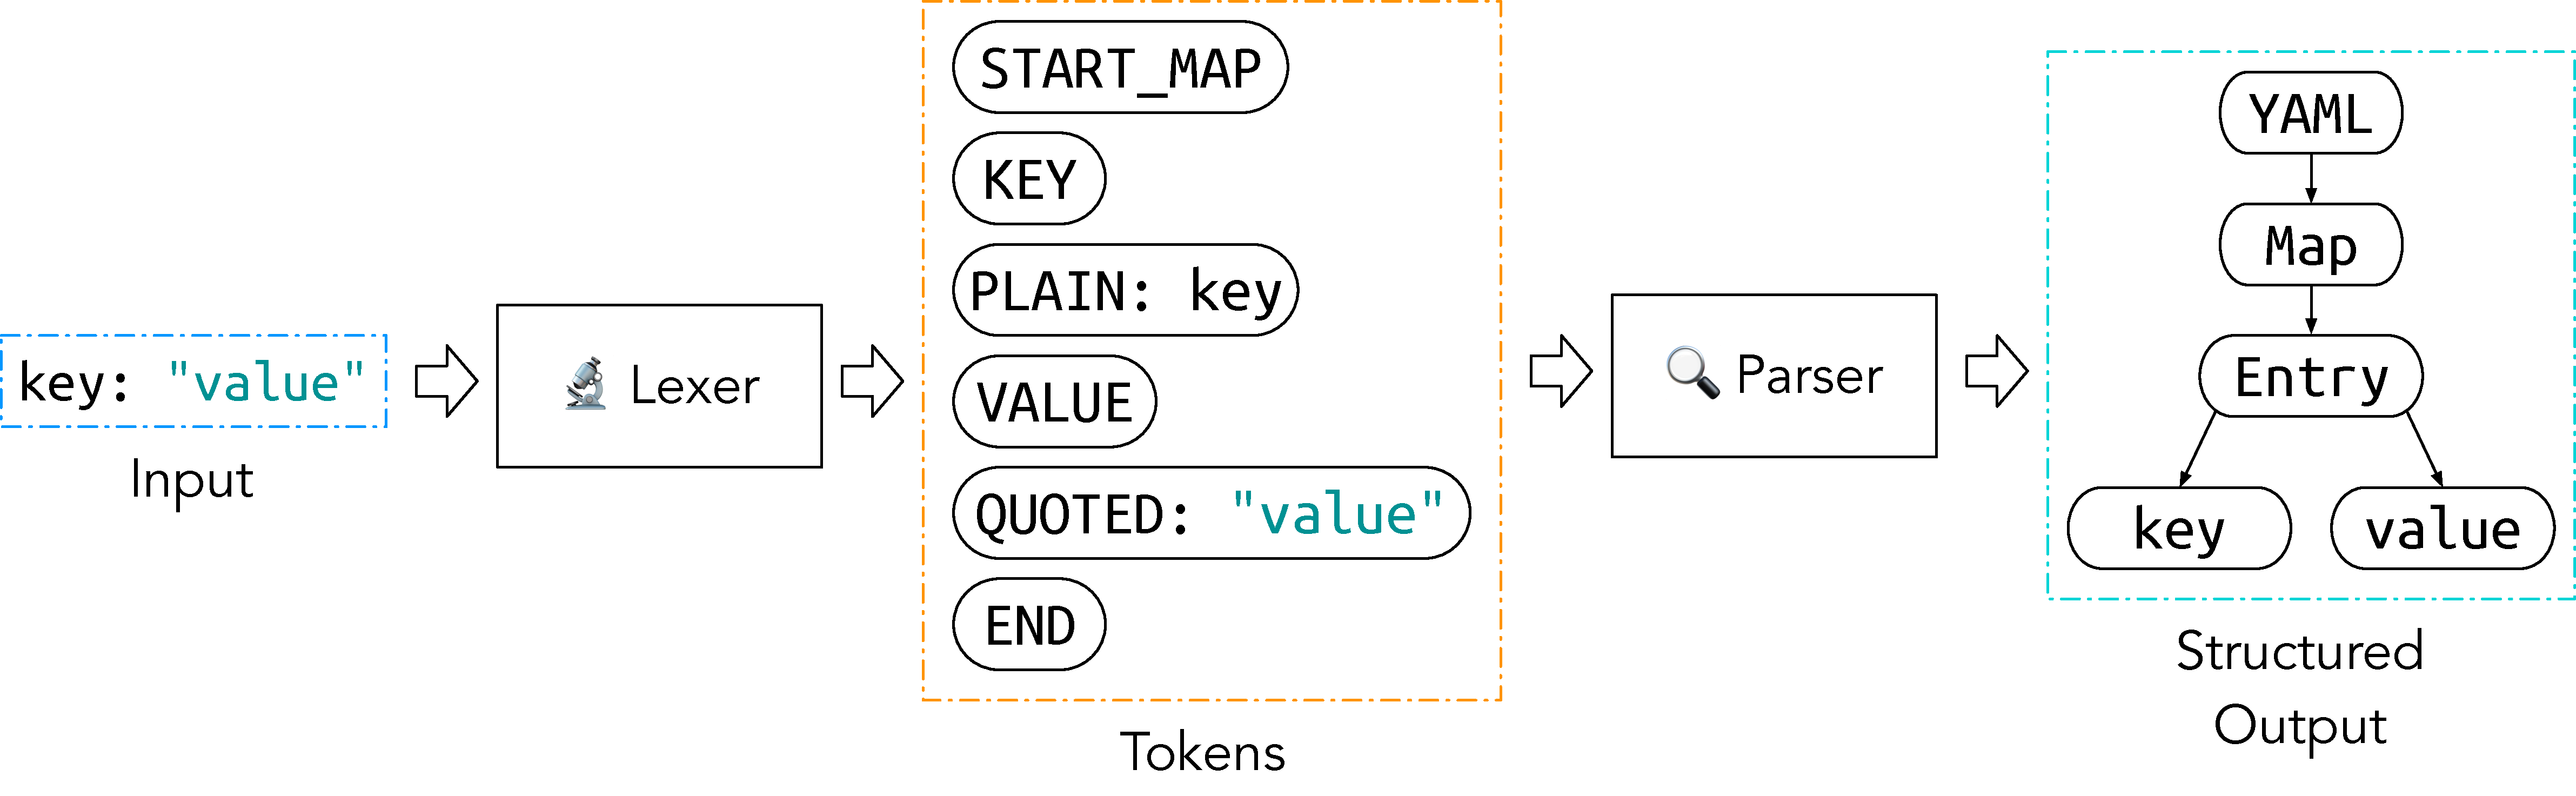
\includegraphics[width=\textwidth]{LexingParsing}
  \caption{A lot of parser engines use two distinct phases (lexing and parsing) to process input.}
  \label{fig:lexing_parsing}
\end{figure}

Unlike \gls{ANTLR}, Bison and YAEP, the library \href{https://github.com/taocpp/PEGTL}{PEGTL} does not use a separate lexing phase. Instead the \gls{PEGTL} parses the input in one sweep using C++ templates to combine simple matching functions into more elaborate parsers. The process of combining parsers this way is also known under the name “parser combinators” (see also Section “\nameref{sec:parsing}”). Besides the possibility to create \emph{custom matching function}, the library also supports:

\begin{itemize}
  \item \emph{custom actions} to react to matched input, and
  \item \emph{custom state} to store contextual data.
\end{itemize}

Using the three features above we were able to create a \gls{PEG} parser plugin called \LinkYAyPEG{} that uses grammar rules that are similar to the ones described by the \href{http://yaml.org/spec/1.2/spec}{YAML specification}.

The translation of some of the rules from the \glstext{YAML} specification to \gls{PEGTL} rules was trivial. For example, the rule:

\begin{ccode}
ns-plain-first(c) ::= ( ns-char - c-indicator )
                    | ( ( "?" | ":" | "-" )
                        /* Followed by an ns-plain-safe(c)) */ )
\end{ccode}

translates to the following code:

\begin{cppcode}
struct ns_plain_first : sor<seq<not_at<c_indicator>, ns_char>,
                            seq<one<'?', ':', '-'>,
                                at<ns_plain_safe>>> {};
\end{cppcode}

. The rule \cc{sor} represents ordered choice, meaning that it tries to match it’s template arguments:

\begin{enumerate}
  \item \cc{seq<not_at<c_indicator>, ns_char}, and
  \item \cc{seq<one<'?', ':', '-'>, at<ns_plain_safe>>}
\end{enumerate}

in order. It succeeds if one of the argument matches, or fails if all of them fail. The rule \cc{seq} on the other hand tries to match all its template arguments in sequence and either succeeds, if all of them succeed, or fails, if one of them fails. The rules \cc{at} and \cc{not_at} represents the \gls{PEG} predicates \cc{&} and \cc{!}. The predicate rule \cc{at} (\cc{&}) succeeds if the current input matches the given input and fails if it does not. The predicate rule \cc{not_at} behaves exactly opposite. Neither of these predicates consumes any input. The only remaining rule is \cc{one}, which tries to match any of the given characters, \cc{'?'}, \cc{':'} or \cc{'-'} in our example.

While translating the rule \cc{ns-plain-first(c)} was not that hard, other rules that contained nested contextual data such as:

\begin{ccode}
l+block-sequence(n) ::= ( s-indent(n+m) c-l-block-seq-entry(n+m) )+
                        /* For some fixed auto-detected m > 0 */
\end{ccode}

proved more difficult to express in the \gls{PEGTL}. To translate these kind of rules we added a custom state that contains a stack for the indentation (the values \cc{n} and \cc{n+m} above). In the  example above a metarule puts the value \cc{n+m} on the stack before the parser tries to match \cc{s-indent(n+m)} and \cc{c-l-block-seq-entry(n+m)} multiple times. Afterwards the metarule removes the last value from the stack leaving the previous value \cc{n}. We called the general metarule that makes this possible \cc{with_updated_state}:

\begin{cppcode}
  template <typename UpdateStateRule,
            typename RevertStateRule,
            typename... Rules>
  struct with_updated_state :
  seq<UpdateStateRule,
      sor<seq<Rules...>,
          seq<RevertStateRule, failure>>,
      RevertStateRule> {};
\end{cppcode}

. As we can see above \cc{with_updated_state} first invokes the rule \cc{UpdateStateRule} to update the state, then it tries to match a sequence of all rules stored in the template parameter pack \cc{Rules}. Depending on the success of \cc{seq<Rules>},

\begin{enumerate}
  \item the rule \cc{with_updated_state} either applies \cc{RevertStateRule} (third argument of outermost \cc{seq}) and succeeds, if \cc{seq<Rules...>} succeeds, or
  \item it applies \cc{RevertStateRule} and fails (second argument of \cc{sor}) if \cc{seq<Rules...>} failed.
\end{enumerate}

We used \cc{with_updated_state} to create rules that update nested versions of the indentation (\cc{n} and \cc{m} in the \glstext{YAML} spec) and context (\cc{c} in the \glstext{YAML} spec). Using this approach we were able to translate all \glstext{YAML} rules for our subset.

For the conversion of the parsed data to a \cc{KeySet} we used the parse tree facility provided by \gls{PEGTL}. The whole parse tree contains many unnecessary nodes. Fortunately \gls{PEGTL} supports parse tree selection and tree rewriting. These features allowed us to keep the parse tree simple. We then use custom tree walking code to walk this tree, invoking a listener at certain nodes, to create a \cc{KeySet}. This approach is very similar to the one we used for the \LinkYAwn{} plugin (see Section “\nameref{sec:earley_parser}”).

\subsection{Parser Combinator}

As described in the previous section “\nameref{sec:peg_parser}” we already used a parser combinator library to create a parser for our basic \glstext{YAML} subset. Initially we also wanted to use a second parser combinator library called \href{https://github.com/orangeduck/mpc}{mpc}. However we decided against using mpc, since

\begin{itemize}
  \item the parser engine \href{https://github.com/orangeduck/mpc#does-mpc-support-unicode}{only supports ASCII} encoded data,
  \item requires manual memory management – mpc is written in C – and
  \item does not provide built-in support for advanced features such as tree selection
\end{itemize}

. In the end we did not think the effort to create yet another parser was worth the time, since at least in theory \gls{PEGTL} seemed to be the better choice.

\subsection{Augeas Lens}

Augeas~\cite{lutterkort2008augeas} is a tool that uses so-called
lenses to edit configuration data. The main advantage of lenses is that they
handle both the parsing and writing process. Since Elektra already includes a
plugin for Augeas~\cite{berlakovich2016universal}, it sounds like a \glstext{YAML}
lens is the ideal tool to convert \glstext{YAML} data to a \cc{KeySet}. In reality there
are multiple problems with this approach. Besides the issues mentioned by
\citeauthor{berlakovich2016universal} in his bachelor thesis~\cite{berlakovich2016universal}, one of
the main problems is that \glstext{YAML} is a context-sensitive
language~\cite{lutterkort2017augeas}, while Augeas offers only full support for
regular languages. With this in mind we tested the official \glstext{YAML} lens with Elektra’s \href{https://www.libelektra.org/manpages/kdb}{\cc{kdb} tool}. Since even the conversion of a single single key-value pair failed, we used the tool \href{https://github.com/raphink/augeas-sandbox/blob/master/augcheck}{\cc{augcheck}} to make sure the \glstext{YAML} lens is able to parse our example data. This tool showed us that the \href{https://github.com/hercules-team/augeas/blob/d555a995a06ac81cab62d016d6eaff8a7ba64a2e/lenses/tests/test_yaml.aug}{YAML lens} currently supports nested mappings, such as

\begin{yamlcode}
  root:
    key: value
\end{yamlcode}

but is unable to handle a non-nested mapping:

\begin{yamlcode}
  key: value
\end{yamlcode}

and other simple data. With the current state of the \glstext{YAML} lens and the problems of the Augeas plugin in mind, we decided to not look any further into developing an Augeas lens for our \glstext{YAML} subset.

\section{Additional Plugins}

While most of the problems of adding a \glstext{YAML} storage plugin deal with the parsing process itself, there are other issues we handled using additional plugins. Elektra’s plugin system allows us to use multiple plugins in conjunction as part of a so-called \emph{backend} (see also section~“\nameref{sec:plugins}”).

\subsection{Base64}
\label{sec:base64}

One of the first plugins we used to improve the \glstext{YAML} support of Elektra was the \href{https://www.libelektra.org/plugins/base64}{Base64} plugin of Peter Nirschl~\cite{nirschl2018crypto}. The plugin en- and decodes binary values using the Base64 algorithm~\cite{josefsson2006base16}.

Since Elektra supports values containing binary data, we can use the Base64 plugin to encode this data and store it using ASCII values in a \glstext{YAML} file. However, the plugin used a common prefix to mark base64-encoded data. For example, if we want to store the decimal numbers 104 (0x68) and 105 (0x69), then the plugin would encode these values as \code{aGk=} and add the prefix \code{@BASE64}. The resulting value would then be \yaml{"@BASE64aGk="}. In \glstext{YAML} a value should not contain a prefix. Instead \glstext{YAML} marks base64 encoded data with the tag (data type) \yaml{!!binary}. We therefore need to store the two values above as \yaml{!!binary "aGk="} in a \glstext{YAML} file. For this purpose we added a new mode to the Base64 plugin.

The new \emph{meta mode} uses metadata to mark a key-value pair that contains a base64-encoded value. Instead of a prefix Base64 adds a meta-key \code{type} with the value \code{binary}. Figure~\ref{fig:base64} shows an example, where Elektra uses the Base64 plugin to encode and decode the bytes 0x68 and 0x69 (code points for the ASCII string \yaml{hi}).

We should mention here that we only added support for the Base64 encoded data to the \LinkYAMLCPP{} plugin, since we decided to not support tags for our \glstext{YAML} subset (see Section “\nameref{sec:discussion_decision}”).

\begin{figure}
  \centering
    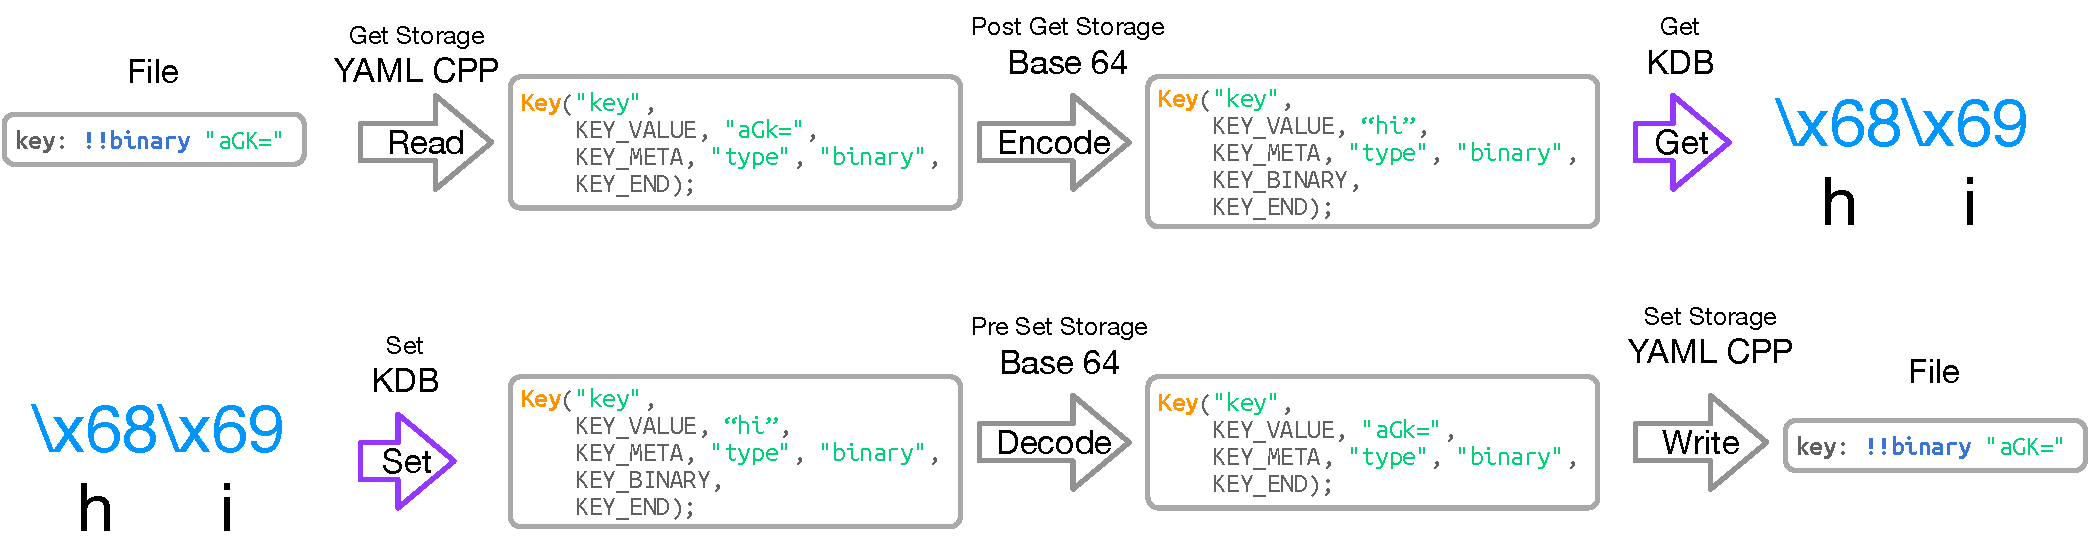
\includegraphics[width=\textwidth]{Base64}
  \caption{The Base64 plugin decodes and encodes binary data.}
  \label{fig:base64}
\end{figure}

\subsection{Directory Value}

We already described the problem of storing a value in a non-leaf (directory) \cc{Key} in the Section~“\nameref{sec:mapping_elektra_yaml}”. Since the problem is independent of the parser engine and also relevant to other plugins, we implemented the functionality in a plugin named \href{http://libelektra.org/plugins/directoryvalue}{Directory Value}.

The Directory Value plugin adds an additional \cc{Key} with the prefix \yaml{___dirdata} for every non-array \cc{Key} that has children and contains a value in the \code{set} direction (position \code{preset}). For example, for the \cc{KeySet} shown in Figure~\ref{fig:keyset_large}, the plugin adds the \cc{Key}

\begin{itemize}
  \item \code{user/yaml/bloc/\_\_\_dirdata} and
  \item \code{user/yaml/bloc/party/\_\_\_dirdata}.
\end{itemize}

The plugin then moves the data stored in the parent \cc{Key} to the newly created \cc{Key}.

\begin{figure}[H]
  \centering
  \begin{subfigure}[t]{.4\textwidth}
    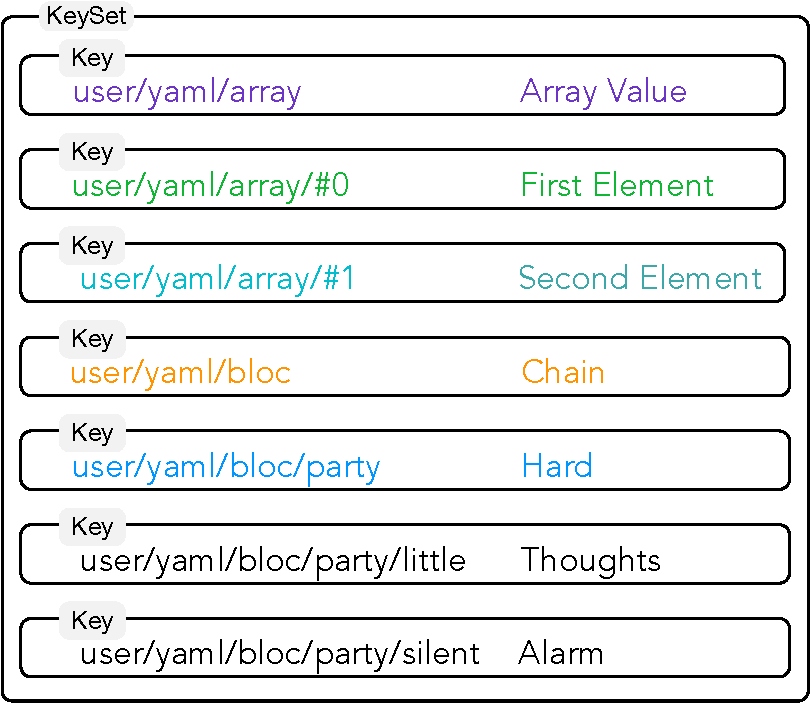
\includegraphics[width=\linewidth]{KeySetLarge}
    \caption{We use the \cc{KeySet} above as input for the Directory Value plugin at the \code{preset} position.}
    \label{fig:keyset_large}
  \end{subfigure}
  \qquad
  \begin{subfigure}[t]{.48\textwidth}
    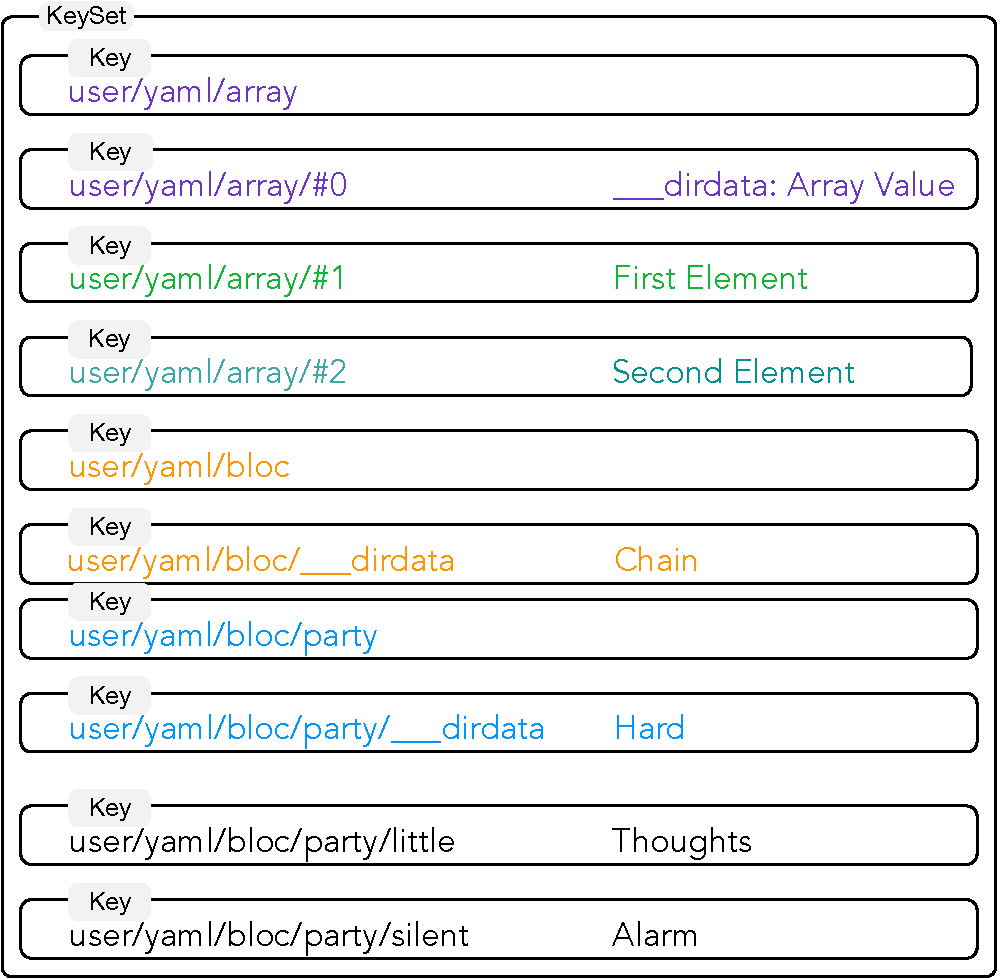
\includegraphics[width=\linewidth]{KeySetLargeExtended}
    \caption{The \cc{KeySet} above shows the result of the conversion at the \code{preset} position.}
    \label{fig:keyset_large_extended}
  \end{subfigure}
  \caption{The Directory Value plugin adds data at the position \code{preset} (\ref{fig:keyset_large_extended}) and then restores the original data (\ref{fig:keyset_large}) at the position \code{postget}.}
\end{figure}

In addition, the plugin inserts a new \cc{Key} for every array parent that stores a (non-binary) value at the first position of the array. In our example, the plugin adds a new \cc{Key} with the value \code{\_\_\_dirdata: Array Value} at the first position of \code{user/yaml/array} and increases the index of all other array elements by one.

Figure~\ref{fig:keyset_large_extended} shows the \cc{KeySet} after the whole conversion at the position \code{preset}. This \cc{KeySet} is also the input for the Directory Value plugin at the position \code{postget}.

\subsection{\glstext{YAML} Smith}

Elektra’s storage plugins need to both:

\begin{enumerate}
  \item convert a configuration file format to a \cc{KeySet}, and
  \item convert a \cc{KeySet} to a configuration file format.
\end{enumerate}

Since the second task is always the same, regardless of the parser library we use, we created a plugin called \href{http://libelektra.org/plugins/yamlsmith}{YAML Smith} that takes care of this task.

This plugin first determines all leaf keys of a \cc{KeySet}. After that it counts the levels of the parent key so it knows how many levels it has to skip for each leaf. The plugin then iterates over each leaf key.

For every leaf key the plugin iterates over each level of the name. First it skips all levels of the parent key. After that it skips all levels of the prefix it shares with the key that came before. In this process it adds a constant amount of spaces for each of the levels to an initially empty string and stores the result in a variable called \cc{indent}. Now the plugin adds each remaining level of the key in its own line. To do that it first writes the content of \cc{indent}, then adds the current part of the key, and after that the appropriate marker, either \yaml{-} for an sequence, or \yaml{:} for a map. For each written level of the key the plugin increases \cc{indent} for the next key part. In the last step for a specific leaf key, the plugin adds another newline, the current indentation and finally writes the value of the key in double quotes.
